\section{時間分解能}
時間分解能は検出器が粒子通過の時刻を正確に測定する能力のことである。%検出する際に、どのくらいの時間幅で測定できるかを表す指標となる。
時間分解能が向上することで、光速で飛んでくる荷電粒子の飛跡を細かく測定することができる。
LGAD検出器の時間分解能$\sigma_{\rm{t}}$を決定する要素は、タイムウォーク$\sigma_{\rm{tw}}$、ジッター$\sigma_{\rm{j}}$、ランダウノイズ$\sigma_{\rm{L}}$の3つが大きく影響すると考えられている。
式\ref{eq_TimingResolution} に示すように、時間分解能は各要素の2乗和の式で表すことができ、それぞれの影響を小さくすることで時間分解能を向上することができる。
\begin{equation}
    {\sigma_{\rm{t}}}^2 = {\sigma_{\rm{tw}}}^2 + {\sigma_{\rm{j}}}^2 + {\sigma_{\rm{L}}}^2
    \label{eq_TimingResolution}
\end{equation}

\subsection{タイムウォーク}
図\ref{fg:TimeWalk} に示すように、タイムウォークとは一定の閾値を設定して到達時間を測定したときに、信号の大きさによって到達時間にばらつきが生じてしまうことをいう。
入射した粒子が検出器内で落とすエネルギーの違いによって波形に違いが生じる。
図\ref{fg:TimeWalk} を見ると大きい信号の方が、小さい信号と比べて到達時間が早くなることがわかる。
図\ref{fg:TimeWalk_50} に示すようにタイムウォークは信号の大きさが異なっても、
信号波高に対して50%の位置に閾値を設定するconstant fraction方式を使用することで、その影響を抑制できる。

\begin{figure}[h]
    \begin{minipage}[b]{0.5\linewidth}
        \centering
        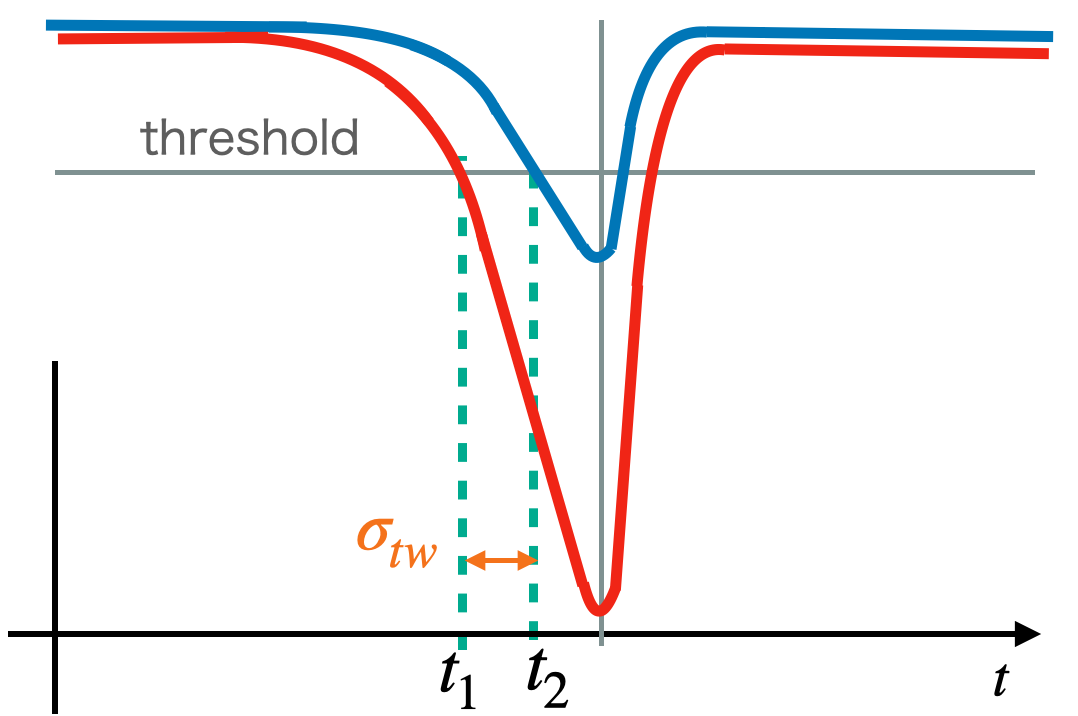
\includegraphics[width=6cm]{fig/ch3/TimeWalk.png}
        \subcaption{一定の閾値のタイムウォークの影響}
        \label{fg:TimeWalk}
    \end{minipage}
    \begin{minipage}[b]{0.5\linewidth}
        \centering
        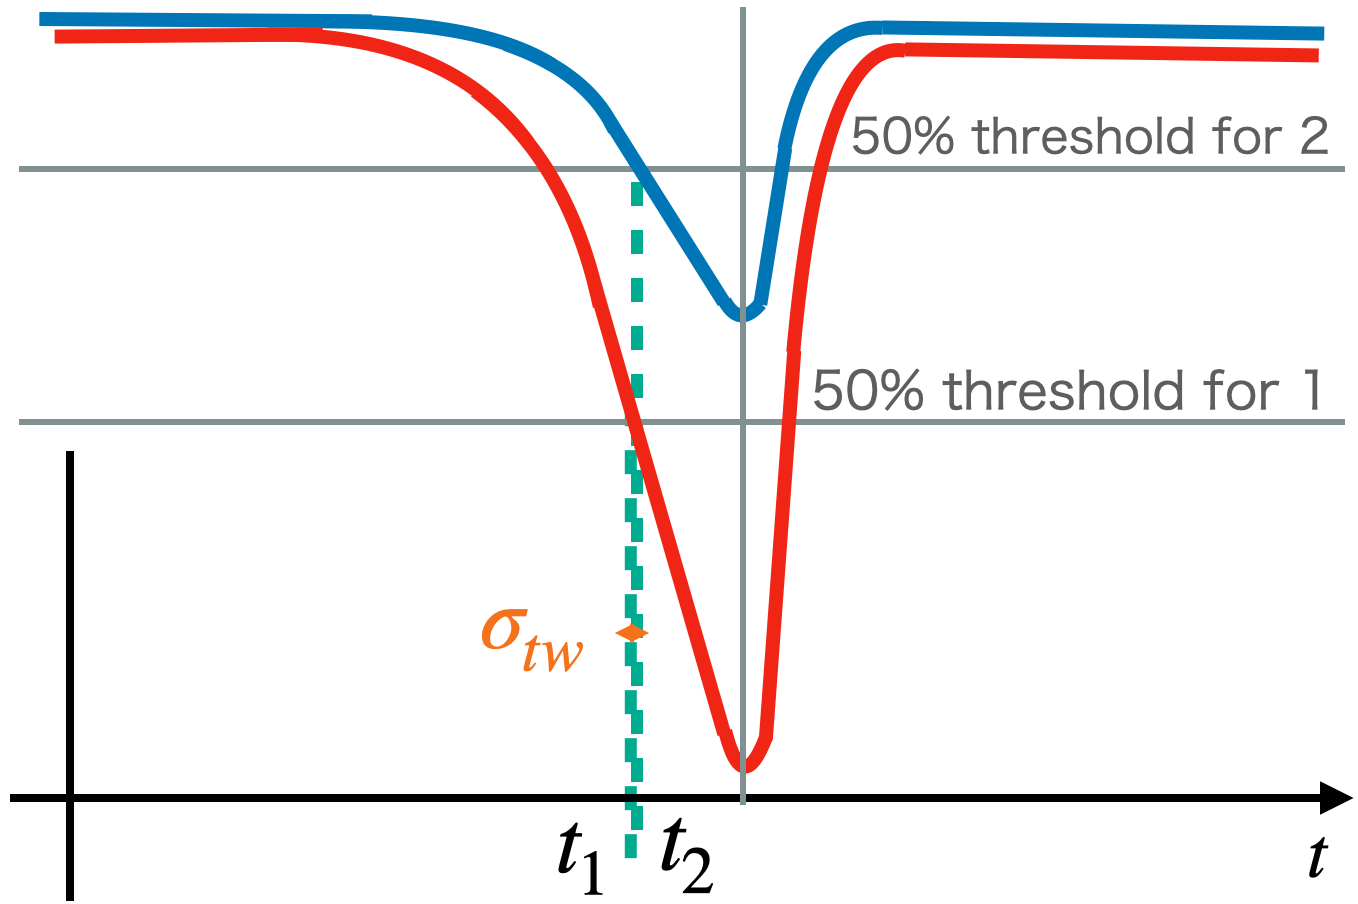
\includegraphics[width=6cm]{fig/ch3/TimeWalk_50.png}
        \subcaption{波高の50%を閾値としたタイムウォークの影響}
        \label{fg:TimeWalk_50}
    \end{minipage}
    \caption[タイムウォークの影響]{タイムウォークの影響\\(a)が一定の閾値を設定したときのタイムウォークで(b)が波高の50%を閾値とした時のタイムウォーク\\波高の50%の時間を到達時間とすることで、タイムウォークの影響を抑制できる。}
\end{figure}


\subsection{ジッター}
図\ref{fg:Jitter} に示すように、ジッターとは測定回路にのるノイズによって到達時間に違いが生じてしまうことをいう。
ジッターは 式\ref{eq_Jitter_1} のように評価することができると考えられている。
$\sigma_{\rm{j}}$がジッター、$\sigma_{\rm{n}}$がノイズ、$\frac{dV}{dt}$が 信号の傾きを示している。
\begin{align}
    \sigma_{\rm{j}} & = \frac{\sigma_{\rm{n}}}{\left|\frac{dV}{dt}\right|} \label{eq_Jitter_1}\\
             & = \frac{\sigma_{\rm{n}}}{\left|\frac{S}{t_{\rm{r}}}\right|} \notag\\
             & = \frac{t_{\rm{r}}}{\left|\frac{S}{\sigma_{\rm{n}}}\right|} \label{eq_Jitter_2}
\end{align}
%\begin{equation}
%    \sigma_{\rm{j}} & = \frac{\sigma_{\rm{n}}}{\left|\frac{dV}{dt}\right|} 
%    \label{eq_Jitter_1}
%            % & = \frac{\sigma_n}{\left|\frac{S}{t_r}\right|} \notag\\
%            % & = \frac{t_r}{\left|\frac{S}{\sigma_n}\right|} \label{eq_Jitter_2}
%\end{equation}
この傾きは信号の大きさ$S$と、立ち上がり時間$t_{\rm{r}}$を用いることで、式\ref{eq_Jitter_2} の分母の形のように表すことができる。
この式から、ジッターは信号ノイズ比(S/N)が大きい場合と、立ち上がり時間が早い場合に小さくなることがわかる。
LGAD検出器は増幅層の効果によって、信号が大きく、立ち上がり時間が早いため、増幅層が無い検出器と比較してジッターが小さくなる。
%本実験では、このジッターの 式\ref{eq_Jitter} が実際にどのくらい正しいのかを信号の大きさ、ノイズ、立ち上がり時間、ジッターを測定することで、定量的に評価する。

\begin{figure}[h]
    \centering
    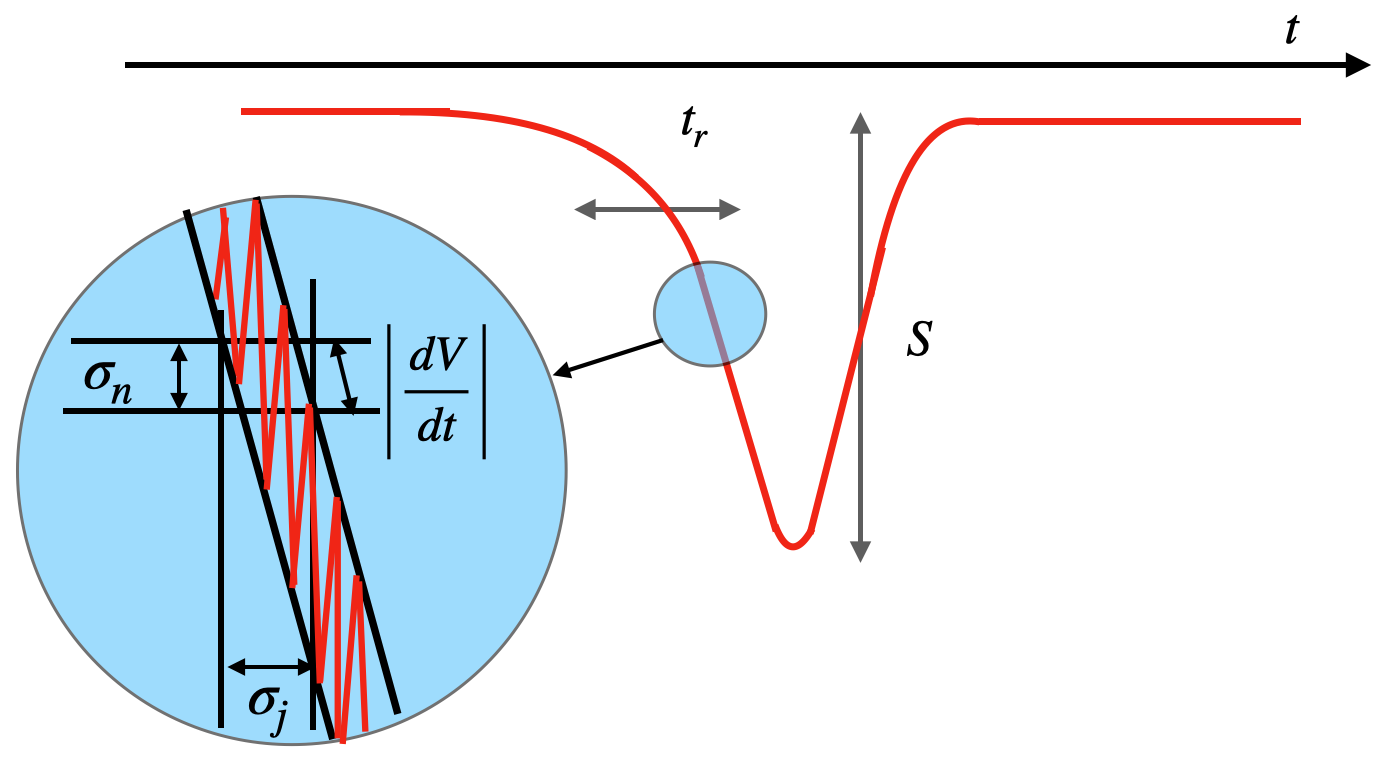
\includegraphics[width=10cm]{fig/ch3/Jitter.png}
    \caption[ジッターの影響]{ジッターの影響\\ノイズにより到達時間にばらつきが生じる。}
    \label{fg:Jitter}
\end{figure}

\subsection{ランダウノイズ}
図\ref{fg:Landaunoise} は荷電粒子が検出器内にエネルギーを落とす様子を示している。
この図のように、荷電粒子がLGAD検出器内に落とすエネルギーは深さによってばらつきがある。
このばらつきはランダウ分布に従い、この深さ方向に対する落とすエネルギーの違いによって、電荷が電極に誘起される時間にばらつきが生じる。
このような影響をランダウノイズを呼ぶ。
%赤外線パルスレーザーを使用すると、1つの光子が落とすエネルギーは深さ方向にばらつきがあるが、検出器内に入射する光子の数が非常に多いため、あたかも
%エネルギー損失が一様な粒子を模擬することができる。そのため、ランダウノイズの影響が少ない状況で時間分解能を測定することができる。

\begin{figure}[h]
    \centering
    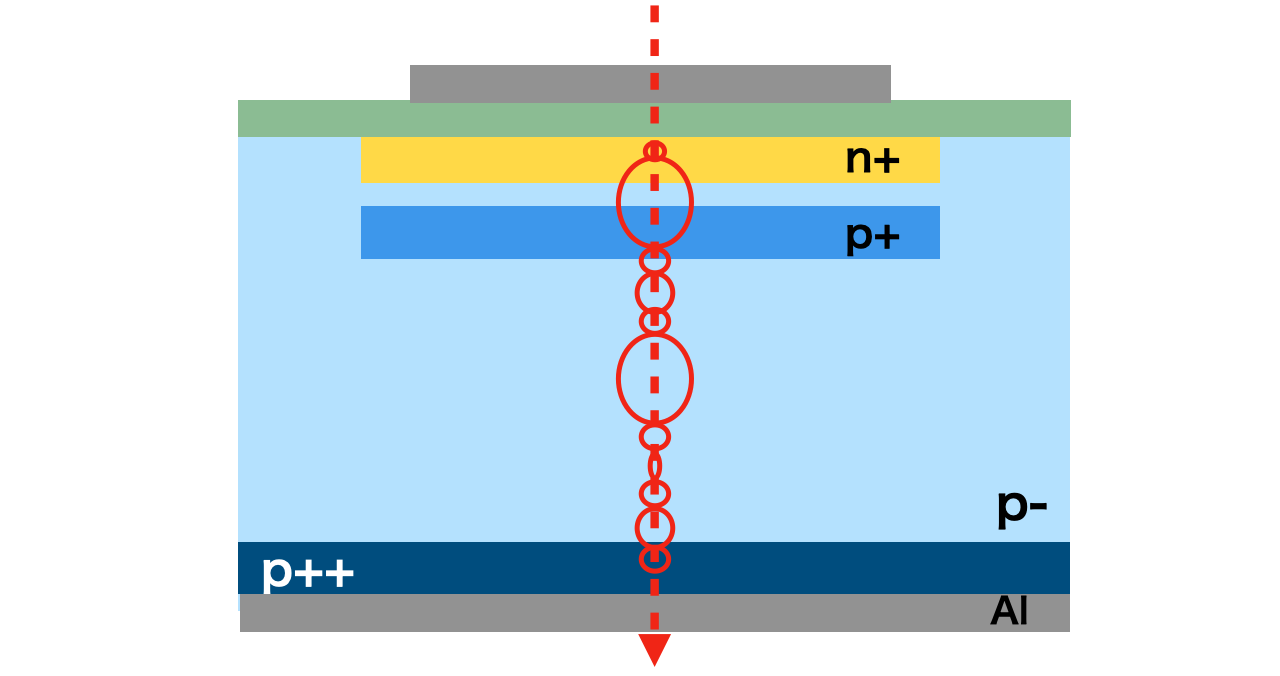
\includegraphics[width=10cm]{fig/ch3/Landaunoise.png}
    \caption[ランダウノイズの影響]{ランダウノイズの影響\\赤丸が荷電粒子が落とすエネルギーの大きさを示している。}
    \label{fg:Landaunoise}
\end{figure}